% 1977 年湖南株洲卷第 14 题：等腰△ABC 内接于圆，A 为顶点，割线 A-D-E 交 BC 于 D、
% 交外接圆于 E，BE 连虚线（按源卷第 7 页布局）
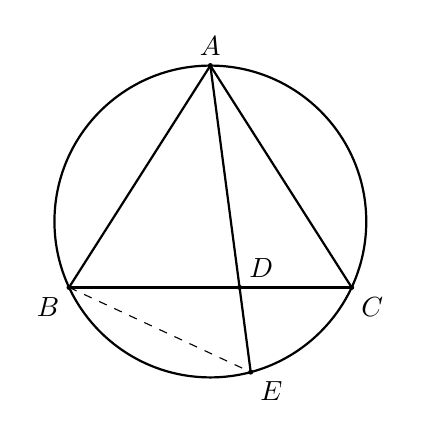
\begin{tikzpicture}[scale=0.66]
  \draw[thick] (0,0) circle (3);
  \coordinate (A) at (90:3);
  \coordinate (B) at (205:3);
  \coordinate (C) at (335:3);
  \coordinate (E) at (285:3);
  \coordinate (D) at (0.561,-1.268);
  \draw[thick] (A)--(B);
  \draw[thick] (A)--(C);
  \draw[thick] (B)--(C);
  \draw[thick] (A)--(E);
  \draw[dashed] (B)--(E);
  \fill (A) circle (1.4pt) node[above] {$A$};
  \fill (B) circle (1.4pt) node[below left] {$B$};
  \fill (C) circle (1.4pt) node[below right] {$C$};
  \fill (D) circle (1.4pt) node[above right] {$D$};
  \fill (E) circle (1.4pt) node[below right] {$E$};
\end{tikzpicture}
